\begin{titlepage}

    \begin{tikzpicture}[remember picture, overlay]
        \def\radius{8mm}      % Circle radius
        \def\rayLength{600mm} % Length of rays
        \def\angleOffset{130} % Offset of rays
        \def\FOVAngle{120}    % Field of View angle (in degrees)
        \def\FOVRange{60mm}   % Field of View range (distance from the center)

        \newcommand{\drawRay}[2]{
            \draw[line width=0.8pt, dotted, black] (center)++(#2+\angleOffset:\radius) --++ (#2+\angleOffset:#1);
        }

        % Define center of the circle
        \coordinate (center) at ([xshift=45mm, yshift=-62mm]current page.center);

        % Draw the circle
        \draw[line width=1.5pt, black] (center) circle [radius=\radius];

        \def\long{600mm}

        \drawRay{118mm}{0}
        \drawRay{\long}{18}
        \drawRay{\long}{36}
        \drawRay{\long}{54}
        \drawRay{092mm}{72}
        \drawRay{059mm}{90}
        \drawRay{\long}{108}
        \drawRay{\long}{126}
        \drawRay{\long}{144}
        \drawRay{\long}{162}
        \drawRay{\long}{180}
        \drawRay{\long}{198}
        \drawRay{\long}{216}
        \drawRay{\long}{234}
        \drawRay{\long}{252}
        \drawRay{\long}{270}
        \drawRay{\long}{288}
        \drawRay{118mm}{306}
        \drawRay{115mm}{324}
        \drawRay{123mm}{342}


        % Draw the field of view (FOV)
        \def\FOVStartAngle{\angleOffset+\FOVAngle/2}  % Start of FOV angle
        \def\FOVEndAngle{\angleOffset-\FOVAngle/2}    % End of FOV angle

        % Draw the two lines defining the FOV
        \draw[thick, black, line width=1.0pt] (center)++(\FOVStartAngle:\radius) -- ++(\FOVStartAngle:\FOVRange);
        \draw[thick, black, line width=1.0pt] (center)++(\FOVEndAngle:\radius) -- ++(\FOVEndAngle:\FOVRange);

        % Draw the arc connecting the two lines
        \draw[thick, black, line width=1.0pt] (center)++(\FOVStartAngle:\FOVRange+\radius) arc (\FOVStartAngle:\FOVEndAngle:\FOVRange+\radius);

    \end{tikzpicture}

    % \begin{textblock*}{\textwidth}(7cm, 20.2cm)
    %     \centering
    %     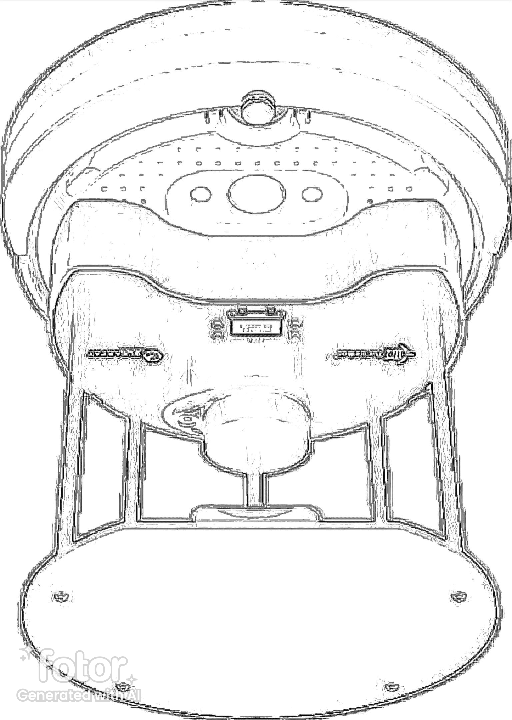
\includegraphics[width=0.12\textwidth]{figures/tb4_sketch.png}
    % \end{textblock*}

    
\includegraphics[width=0.3\textwidth]{figures/sdu_logo.png} \\[10mm]
    % \textsc{University of Southern Denmark} \\[5mm]

    {\Huge \textbf{Coordinated Robot Search}} \\[0.5cm]
    {\Large \textbf{Bachelor's Thesis in Robot Systems}} \\[3mm]
    \noindent\rule{\textwidth}{1pt} \\[15mm]
    {\Large \textbf{Mathias B. Christiansen}} \\[-1mm]
    {\small 205400} \\
    {\Large \textbf{Balder W. Holst}} \\[-1mm]
    {\small 203024}

    \vfill


    {\large
        \textbf{Supervisor: Leon Bodenhagen} \\
        \textbf{Co-supervisor: Roberto de Nóbrega} \\[3mm]
    }

    {\large
        \textbf{Submission Date: 02/06-2025}
    } \\[2mm]

    \textit{Character Count: 70854} \\[-19mm]

\end{titlepage}
